\chapter{Appendices}

\section{Social Networks and Corruption}

\subsection{Description of iWiW data}
\label{SI:iwiwappendix}
In line with previous work on iWiW we filtered the data used in our analysis. We use the data from the network at its peak activity in 2012. Out of roughly 4.5 million user accounts, we dropped the roughly 500,000 accounts with location outside of Hungary. We follow Lengyel et al.~\cite{lengyel2015geographies}, we dropped the 193 users with more than 10,000 connections, arguing that such a large number of connections cannot represent social ties. We argue that this cutoff balances two concerns: it excludes those accounts with so many connections that it brings into question the nature of its connections, and we avoid truncating the tail of the distribution of social connectivity too much, allowing for sociality to range over several orders of magnitude. Many approaches to detect ``fake'' accounts in social network use the degree of a node as an important input~\cite{cao2012aiding}. 

In Plot A of Figure~\ref{fig:iwiw_robustness} we plot the sensitivity of fragmentation and diversity to the maximum degree threshold. If we discard all users with more than 100 connections (compared to the 10,000 connection cutoff we use in our paper), fragmentation would be significantly higher and diversity significantly lower than the versions we use in the paper. However this is not a reasonable cutoff as nearly 10\% of users have more than 500 connections (see Plot B, Figure~\ref{fig:iwiw_robustness}). The settlement fragmentation and diversity measures are within 5\% of the versions we use in the paper if the threshold is set at 500, 1000, or 2000 connections.  



In Figure~\ref{fig:iwiw_stats} we show the relationship between settlement population and the number of iWiW users listing their location in the settlement, and the share of the population registered to iWiW. As mentioned in the text, user privacy is a key concern. The anonymized iWiW data was made available to a consortium of researchers in Hungary, each of whom signed a non-disclosure agreement (NDA) to use the data for research purposes only. As a result, only settlement level aggregated data can be shared. 

\begin{figure}[b]
\centering
  \includegraphics[width=\textwidth]{images/iwiw/robustness_tests.pdf}
  \caption[Sensitivity of social capital network measures to thresholds.]{A) The sensitivity of diversity and fragmentation to changing the maximum degree threshold, relative to the 10,000 degree threshold used in the paper. Error bars represent 95\% confidence intervals. The measures are within 5\% of the version we use in the paper for cutoffs at or above 500. B) The distribution of user connections on a log scale. Very few users (193) have more than 10,000 connections, while many (405,337) have more than 500.}
  \label{fig:iwiw_robustness}
\end{figure}

\begin{figure}
\centering
  \includegraphics[width=\textwidth]{images/iwiw/pop_rate_dists_cropped.png}
  \caption[iWiW usage distributions.]{A) Settlement population and number of iWiW users plotted on a log-log scale. B) iWiW use rate by settlements.}
  \label{fig:iwiw_stats}
\end{figure}



\subsection{Relationship between fragmentation and diversity}
\label{SI:fragdiv}
Fragmentation and diversity, our measures of bonding and bridging social capital respectively, are positively and significantly correlated ($\rho \approx0.46$). Though fragmentation considers only edges within the settlement and ego diversity includes external edges, both variables measure modularity in the network. However, according to our hypotheses, they are expected to capture different kinds of socialization. We found that despite their positive correlation these features have opposite relationships with our corruption risk measures: high fragmentation is positively and high diversity is negatively correlated with corruption risk. To test whether inter-settlement edges or the ego focus of diversity does more to distinguish the measure from fragmentation we recalculated the diversity considering only edges within the settlement. This alternative ``internal'' diversity measure is weakly correlated ($\rho \approx 0.28$) with fragmentation, and strongly correlated with diversity ($\rho \approx 0.72$). This suggests that both the connections to other settlements and the ego-focus of the diversity measure distinguish fragmented settlements from diverse ones.


\subsection{Model covariates and controls}
\label{appendix:descriptives}

In this appendix section we present the settlement-level variables used as controls in our models. We also report their summary statistics. Note that in our models, we scale all features to have mean 0 and standard deviation 1. Our controls mostly refer to data from 2011, when the last large scale Hungarian census took place and the data are of highest quality. 

\begin{itemize}
\item \textit{Average income per capita (2011)}: Wealthier places tend to be less corrupt~\cite{mungiu2013controlling} as competition for limited resources is expected to create greater incentive to cheat. Data on median income or the income distribution at the settlement level were, to the best our knowledge, not available in Hungary.
\item \textit{Population (log)(2011)}: Larger cities may have different contracting needs, different political and social norms, and different network characteristics.
\item \textit{Number of contracts awarded (log)}: Settlements contracting more frequently may be more experienced and may follow better practices. As more people are involved in contracting, corruption may become more difficult.
\item \textit{Rate of iWiW use (2012)}: The rate of iWiW use both proxies for the economic development of the settlement and controls for differences in observed social network structure resulting from differences in access to the web. Previous work suggests that iWiW users, especially the early adopters, skew young and wealthy~\cite{lengyel2015geographies}.
\item \textit{Average mayoral victory margin}: Measured across three elections (2002, 2006, 2010), this variable proxies for the lack of political competition in the settlement. The absence of political competition has been shown to correlate with corruption~\cite{broms2017procurement}.
\item \textit{Share of population with at least a high school diploma (2011)}: Education is typically correlated with better control of corruption~\cite{rothstein2005all}.
\item \textit{Share of working-age population inactive and unemployment rate (2011)}: Counting the long-term and short-term unemployed respectively, these variables quantify economic stagnation. The economic hardship connected with high unemployment is conjectured to worsen political corruption~\cite{sung2004democracy}.
\item \textit{The minimum travel distance to Budapest, the capital city}: This variable captures the physical isolation of the settlement from the main economic, political, and social hub of the country. Past research has shown that geographic isolation reduces accountability and increases corruption~\cite{campante2014isolated}. 
\item \textit{Share of population over 60 years old (2011)}: This variable controls for the over-representation of the elderly. The elderly are underrepresented on online social networks and tend to use these platforms differently than younger users~\cite{pfeil2009age}.
\item \textit{Whether the settlement has a university (2011)}: This variable controls for the presence of a place of higher education in the settlement, including local branches of universities headquartered elsewhere. this which inflates the number of young people, hence likely iWiW users in the settlement.
\end{itemize}

\begin{table} \centering 
\begin{tabular}{@{\extracolsep{3pt}}lccccc} 
\\[-1.8ex]\hline 
\hline \\[-1.8ex] 
Statistic & \multicolumn{1}{c}{N} & \multicolumn{1}{c}{Mean} & \multicolumn{1}{c}{St. Dev.} & \multicolumn{1}{c}{Min} & \multicolumn{1}{c}{Max} \\ 
\hline \\[-1.8ex] 
Closed procedure or single bid. & 169 & 0.59 & 0.15 & 0.21 & 0.92 \\ 
Average CRI & 169 & 0.28 & 0.04 & 0.16 & 0.40 \\ 
Fragmentation & 169 & 0.32 & 0.04 & 0.16 & 0.46 \\ 
Avg. ego diversity & 169 & 0.35 & 0.07 & 0.20 & 0.51 \\ 
Income/capita (thous. HUF) & 169 & 823.57 & 189.93 & 488.44 & 1,516.55 \\ 
N contracts (log) & 169 & 4.52 & 0.69 & 3.69 & 6.42 \\ 
Population (log) & 169 & 9.72 & 0.89 & 7.66 & 12.24 \\ 
Rate iWiW use & 169 & 0.33 & 0.06 & 0.18 & 0.46 \\ 
Average mayoral victory margin & 169 & 0.15 & 0.14 & 0.00 & 0.64 \\ 
\% high school graduates & 169 & 47.23 & 10.22 & 25.70 & 76.80 \\ 
Distance to Budapest (minutes) & 169 & 114.00 & 54.34 & 22.55 & 228.57 \\ 
Share of population inactive & 169 & 0.30 & 0.04 & 0.20 & 0.40 \\ 
Unemployment Rate & 169 & 0.06 & 0.01 & 0.03 & 0.09 \\ 
Share of population 60+ & 169 & 0.24 & 0.03 & 0.15 & 0.39 \\ 
Has university & 169 & 0.25 & 0.44 & 0 & 1 \\ 
\hline \\[-1.8ex] 
\end{tabular} 
\caption{Descriptive statistics of key settlement-level variables and controls.}
\label{tab:desc}
\end{table} 


\subsection{Model results, diagnostics, and feature importances}

We also present models including only one of the two network measures in Table~\ref{stepwise}. The effect and significance of both features is preserved when the other is excluded. Recall that all variables are standardized with mean 0 and standard deviation 1. This aids interpretation, for example: a one standard deviation increase in the settlement's mayor's average margin of victory increases corruption risk by roughly one quarter of a standard deviation.

The estimated coefficients of the control variables and their levels of statistical significance offer additional insight into the phenomenon of corruption risk. Wealthier settlements are in general less corrupt, though the effect is not significant for CRI. Rate of iWiW use is not related with corruption risk and this does not change when we include the social capital features. The average mayoral victory margin is a highly significant positive predictor of corruption risk. One potential explanation is that mayors, who do not face significant competition do not fear being voted out of office if they are corrupt. Similarly settlements that are far from Budapest, which our models predict to be significantly more corrupt, may be insulated from investigation by the central authorities simply by being out of the spotlight.




\begin{table}
\begin{center}
\ra{.75}
%\setlength\tabcolsep{1pt}
%\begin{tabular}{@{\extracolsep{1cm}}lp{1cm}p{1cm}p{1cm}p{1cm}} 
\begin{tabular}{@{\extracolsep{.3cm}}lr{1cm}r{1cm}r{1cm}r{1cm}} 
\toprule
%\setlength\tabcolsep{2.5pt}
Dependent variable: & \multicolumn{4}{c}{\% Closed or single bid.} \\
\\[-1.8ex] & \multicolumn{1}{c}{(1)} & \multicolumn{1}{c}{(2)} &\multicolumn{1}{c}{(3)} & \multicolumn{1}{c}{(4)} \\ 
\cmidrule{2-5}
 \textbf{\textit{Fragmentation}} &  &  & 0.233$^{**}$ & 0.263$^{***}$ \\ 
 (Bonding social capital) &  &  & (0.099) & (0.097) \\ 
  & & & & \\ 
 \textbf{\textit{Diversity}} &  & $-$0.505$^{***}$ &  & $-$0.553$^{***}$ \\ 
 (Bridging social capital) &  & (0.179) &  & (0.176) \\ 
  & & & & \\ 
 Income/capita & $-$0.262 & $-$0.295$^{*}$ & $-$0.243 & $-$0.277$^{*}$ \\ 
  & (0.169) & (0.166) & (0.167) & (0.162) \\ 
  & & & & \\ 
 N contracts (log) & $-$0.313$^{*}$ & $-$0.359$^{**}$ & $-$0.269 & $-$0.314$^{*}$ \\ 
  & (0.171) & (0.168) & (0.169) & (0.165) \\ 
  & & & & \\ 
 Population (log) & $-$0.180 & 0.083 & $-$0.257$^{*}$ & 0.020 \\ 
  & (0.143) & (0.168) & (0.144) & (0.166) \\ 
  & & & & \\ 
 Rate iWiW use & 0.045 & 0.009 & 0.073 & 0.037 \\ 
  & (0.137) & (0.134) & (0.135) & (0.132) \\ 
  & & & & \\ 
 Mayor victory margin  & 0.278$^{***}$ & 0.259$^{***}$ & 0.276$^{***}$ & 0.255$^{***}$ \\ 
  & (0.089) & (0.087) & (0.088) & (0.086) \\ 
  & & & & \\ 
 \% high school grads & 0.166 & 0.397$^{*}$ & 0.126 & 0.374$^{*}$ \\ 
  & (0.190) & (0.203) & (0.188) & (0.199) \\ 
  & & & & \\ 
 Distance to Budapest & $-$0.021 & $-$0.169 & $-$0.035 & $-$0.198$^{*}$ \\ 
  & (0.104) & (0.114) & (0.102) & (0.112) \\ 
  & & & & \\ 
 Share of pop. inactive & $-$0.797$^{***}$ & $-$0.931$^{***}$ & $-$0.675$^{***}$ & $-$0.805$^{***}$ \\ 
  & (0.229) & (0.229) & (0.232) & (0.229) \\ 
  & & & & \\ 
 Unemployment Rate & 0.239$^{**}$ & 0.253$^{**}$ & 0.247$^{**}$ & 0.262$^{**}$ \\ 
  & (0.118) & (0.115) & (0.116) & (0.113) \\ 
  & & & & \\ 
 \% population 60+ & 0.501$^{***}$ & 0.546$^{***}$ & 0.449$^{***}$ & 0.491$^{***}$ \\ 
  & (0.163) & (0.160) & (0.162) & (0.158) \\ 
  & & & & \\ 
 Has University & 0.351 & 0.198 & 0.449$^{**}$ & 0.294 \\ 
  & (0.220) & (0.222) & (0.221) & (0.221) \\ 
  & & & & \\ 
 Constant & 1.245$^{*}$ & 1.426$^{**}$ & 1.036 & 1.206$^{*}$ \\ 
  & (0.725) & (0.712) & (0.720) & (0.702) \\ 
  & & & & \\ 
\hline \\[-1.8ex] 
Observations & 169 & 169 & 169 & 169 \\ 
Adjusted R$^{2}$ & 0.163 & 0.198 & 0.186 & 0.230 \\ 
F Statistic & 3.967$^{***}$  & 4.460$^{***}$ & 4.207$^{***}$ & 4.859$^{***}$  \\ 
\bottomrule
\end{tabular} 
  \caption[Stepwise regressions predicting municipality corruption risk.]{Stepwise regressions. The effect and significance of the network features are preserved when including them only one at a time. $^{*}$p$<$0.1; $^{**}$p$<$0.05; $^{***}$p$<$0.01.} 
  \label{stepwise}
  \end{center}
\end{table} 
\label{appendix:model_diag}


\begin{figure}
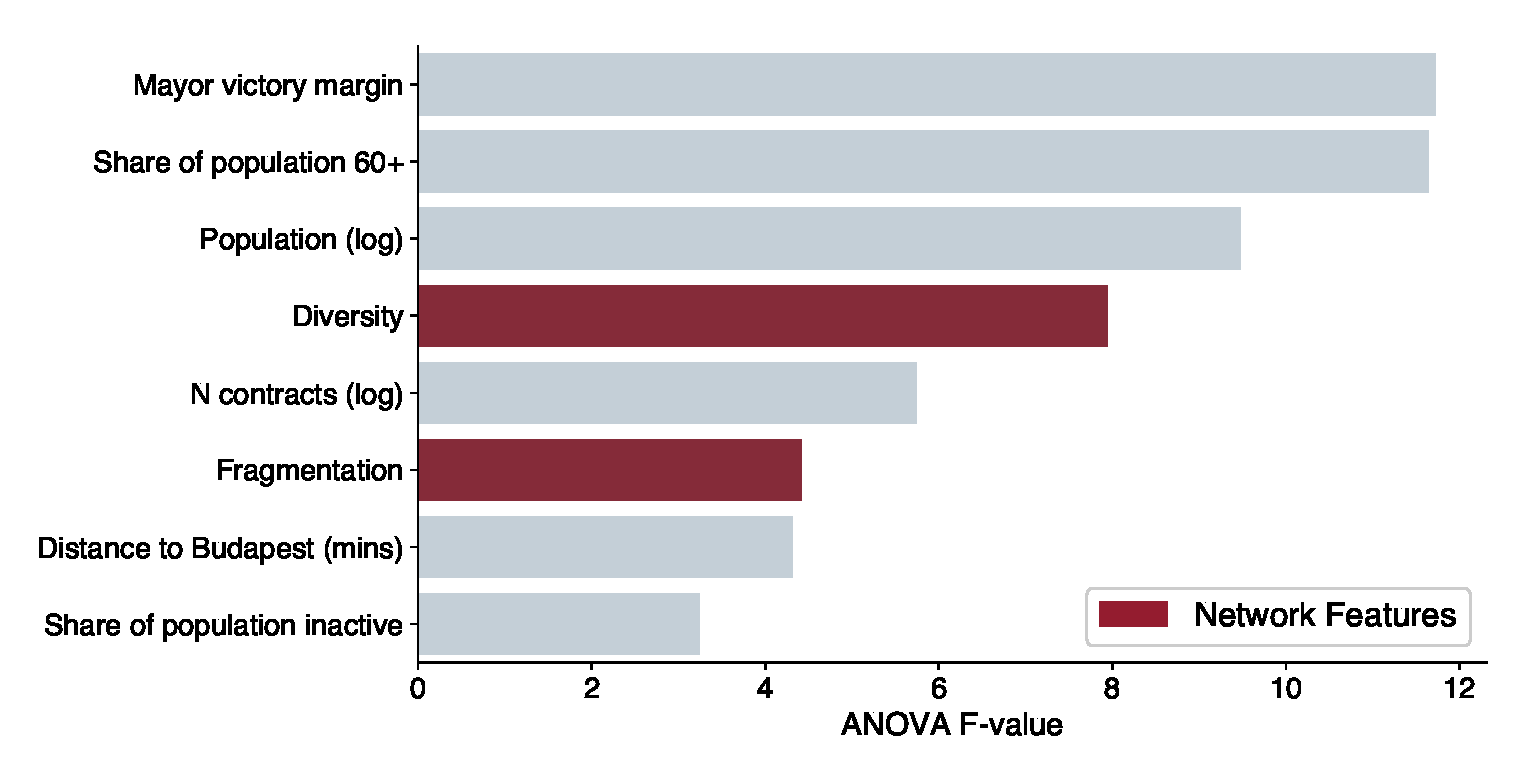
\includegraphics[width=\textwidth]{images/iwiw/feature_importances.eps}
\caption{Analysis of Variance F-test feature importances of OLS regression predicting average settlement CRI. We only include significant features, and highlight the network-based social capital measures.}
\label{fig:feat_imps}
\end{figure}

One potential source of bias in the coefficient estimates of multiple regression models is collinearity among the predictors. We test for multi-collinearity for each predictor using a variance inflation factor (VIF) test, defined as the ratio of variance in the full model over the variance of the single-predictor model. We run this diagnostic for each predictor used in models (2) and (4) in the main text and report the results in Table~\ref{tab:vif}. A popular rule of thumb is that VIF values under 10 denote acceptable levels of correlation between variables~\cite{hair1999analysis}. As it is near our limit, we reran our analyses without the ``Share of population inactive'' control variable, finding no substantive change in our results. The relevant model tables are available on request.

\begin{table}
\begin{center}
\ra{1.1}
\begin{tabular}{ l  l   }\toprule
Predictor & VIF   \\\midrule
\textbf{\textit{Fragmentation}} &1.407\\ 
\textbf{\textit{Diversity}} & 6.337 \\
Income/capita & 5.430 \\ 
N contracts (log)& 3.045  \\
Population (log) & 5.892 \\ 
Rate iWiW use& 2.885 \\
Mayor victory margin & 1.040 \\ 
\% high school grads & 7.106  \\
Share of pop. inactive & 9.899 \\ 
Unemployment Rate & 2.360  \\
Distance to Budapest & 3.068 \\ 
\% population 60+ & 5.442  \\
Has university & 2.192  \\
\bottomrule
\end{tabular}
\caption{VIF scores for model predictors.}
\label{tab:vif}
\end{center}
\end{table}

We show the relative variable importances of Model (6) (column 6 in Table~\ref{tab:ols_regs}), the fully specific model predicting average CRI, using an Analysis of Variance F-test in Figure~\ref{fig:feat_imps}. We include only terms with a significant ANOVA F-test. Though other features have stronger predictive power, the social network features are more useful in predicting corruption risk than economic variables like unemployment, inactivity, and average income.




\begin{table}
\begin{center}
\ra{.75}
%\setlength\tabcolsep{1pt}
%\begin{tabular}{@{\extracolsep{1cm}}lp{1cm}p{1cm}p{1cm}p{1cm}} 
\begin{tabular}{@{\extracolsep{.3cm}}lr{1cm}r{1cm}r{1cm}r{1cm}} 
\toprule
%\setlength\tabcolsep{2.5pt}
Dependent variable: & \multicolumn{2}{c}{\% Closed or single bid.} & \multicolumn{2}{c}{Average CRI} \\
\\[-1.8ex] & \multicolumn{1}{c}{(1)} & \multicolumn{1}{c}{(2)} &\multicolumn{1}{c}{(3)} & \multicolumn{1}{c}{(4)} \\ 
\cmidrule{2-3} \cmidrule{4-5} \\
 \textbf{\textit{Fragmentation}}  &  & 0.143$^{**}$ &  & 0.140$^{**}$ \\ 
 (Bonding social capital)  &  & (0.069) &  & (0.067) \\ 
  & & & & \\ 
\textbf{\textit{Diversity}} &  & $-$0.358$^{***}$ &  & $-$0.440$^{***}$ \\ 
  (Bridging social capital) &  & (0.138) &  & (0.134) \\ 
  & & & & \\ 
Income/capita & $-$0.324$^{**}$ & $-$0.351$^{***}$ & $-$0.323$^{**}$ & $-$0.356$^{***}$ \\ 
  & (0.131) & (0.129) & (0.128) & (0.126) \\ 
  & & & & \\ 
 N contracts (log) & $-$0.389$^{***}$ & $-$0.384$^{***}$ & $-$0.669$^{***}$ & $-$0.672$^{***}$ \\ 
  & (0.118) & (0.118) & (0.116) & (0.115) \\ 
  & & & & \\ 
 Population (log) & $-$0.064 & 0.036 & 0.176 & 0.318$^{**}$ \\ 
  & (0.112) & (0.131) & (0.110) & (0.128) \\ 
  & & & & \\ 
 Rate iWiW use & 0.042 & $-$0.001 & 0.105 & 0.052 \\ 
  & (0.094) & (0.094) & (0.092) & (0.092) \\ 
  & & & & \\ 
 Mayor victory margin & 0.176$^{**}$ & 0.173$^{**}$ & 0.174$^{**}$ & 0.169$^{**}$ \\ 
  & (0.070) & (0.069) & (0.069) & (0.067) \\ 
  & & & & \\ 
 \% high school grads & 0.170 & 0.348$^{**}$ & $-$0.036 & 0.190 \\ 
  & (0.122) & (0.144) & (0.120) & (0.140) \\ 
  & & & & \\ 
 Distance to Budapest & $-$0.089 & $-$0.204$^{**}$ & 0.048 & $-$0.093 \\ 
  & (0.078) & (0.088) & (0.077) & (0.086) \\ 
  & & & & \\ 
 Share of pop. inactive & $-$0.456$^{***}$ & $-$0.440$^{***}$ & $-$0.430$^{***}$ & $-$0.422$^{***}$ \\ 
  & (0.138) & (0.138) & (0.135) & (0.134) \\ 
  & & & & \\ 
 Unemployment Rate & 0.058 & 0.064 & $-$0.017 & $-$0.011 \\ 
  & (0.079) & (0.078) & (0.078) & (0.076) \\ 
  & & & & \\ 
 \% population 60+ & 0.358$^{***}$ & 0.329$^{***}$ & 0.283$^{***}$ & 0.251$^{**}$ \\ 
  & (0.108) & (0.107) & (0.106) & (0.104) \\ 
  & & & & \\ 
 Has University & 0.289 & 0.289 & 0.406$^{**}$ & 0.384$^{*}$ \\ 
  & (0.204) & (0.208) & (0.200) & (0.202) \\ 
  & & & & \\ 
 Constant & 1.561$^{***}$ & 1.540$^{***}$ & 2.642$^{***}$ & 2.652$^{***}$ \\ 
  & (0.463) & (0.464) & (0.453) & (0.451) \\ 
  & & & & \\ 
\hline \\[-1.8ex] 
Observations & 305 & 305 & 305 & 305 \\ 
Adjusted R$^{2}$ & 0.106 & 0.129 & 0.143 & 0.175 \\ 
F Statistic & 4.271$^{***}$ & 4.452$^{***}$ & 5.628$^{***}$  & 5.974$^{***}$  \\ 
\bottomrule
\end{tabular} 
  \caption[Lower inclusion threshold regression robustness test.]{Settlement-level regression results predicting two corruption risk indicators, including all towns issuing at least one contract a year on average from 2006 to 2014. Note that all features are standardized with mean 0 and standard deviation 1. Significance thresholds: $^{*}$p$<$0.1; $^{**}$p$<$0.05; $^{***}$p$<$0.01.} 
  \label{SI:lower_threshold_ols}
  \end{center}
\end{table} 

\newpage


\section{Cartels}

\subsection{Ohio School Milk Data}
In this section of the appendix we report summary statistics about the Ohio school milk market in Table~\ref{tab:app_ohio_summary} and plot the co-bidding networks of the market annually in Figure~\ref{fig:ohio_nets}. We plot the distributions of the sizes of groups detected in the co-bidding network by year in Figure~\ref{fig:oh_group_sizes}.

\begin{table}[]
\ra{1.1}
\begin{tabular}{lccc}
\toprule
Year & \# Contracts & \# Firms & Avg. \# Bidders &   \\ 
\midrule
1981 & 273   & 49 & 1.96 &  \\
1982 & 287  & 43 & 1.96 &\\
1983 & 318   & 46 & 2.01 &  \\
1984 & 339  & 55 & 1.94 &\\
1985 & 357   & 49 & 1.93 &  \\
1986 & 378  & 49 & 2.02 &\\
1987 & 411   & 42 & 1.97 &  \\
1988 & 419  & 41 & 1.83 &\\
1989 & 392   & 40 & 1.76 &  \\
1990 & 331  & 43 & 1.73 &\\
\bottomrule
\end{tabular}
\caption{Summary statistics of the Ohio school milk market by year.}
\label{tab:app_ohio_summary}
\end{table}

\begin{figure}
\centering
\includegraphics[width=\textwidth]{images/cartels/ohio_nets.pdf}
\caption[Ohio school milk co-bidding networks by year.]{Ohio school milk procurement market co-bidding networks, 1981-1990. Red nodes are members of the alleged cartel. For the purposes of visualization we filter out nodes participating in fewer than 5 auctions with other firms. Nodes are placed using a force-layout algorithm, with initial position equal to the final position of the nodes in the previous year.}
\label{fig:ohio_nets}
\end{figure}

\begin{figure}
\includegraphics[width=\textwidth]{images/cartels/ohio_group_sizes.pdf}
\caption{Distributions of detected group sizes from the Ohio school milk contracting data, by year.}
\label{fig:oh_group_sizes}
\end{figure}



\subsection{Georgian Contracting Data}
In Table~\ref{tab:ga_stats_table} we report annual summary statistics on the Georgian public procurement market. In Figure~\ref{fig:ga_group_sizes} we plot the distribution of the sizes of the groups we detected in the Georgian co-bidding network each year.

\begin{table}[]
\ra{1.4}
\begin{tabular}{@{}lccccccc{}}\toprule
Year & \# Contracts & \# Firms & Avg. \# & Share& Total & Avg. Rel. \\
 &  &  & Bidders &Protested & Value(GEL)  & Cost   \\
\midrule
2011 & 17,396   & 3,804 & 1.73 & .003& 1,327,227,101 & .88 & \\
2012 & 18,575  & 4,048 & 1.75 & .004&1,331,025,922& .88 & \\
2013 & 20,230   & 4,399 & 2.03& .012 & 1,665,836,758 & .85 & \\
2014 & 22,122  & 4,884 & 2.02& .014 &1,808,309,559 & .86 &\\
2015 & 26,033   & 5,600 & 2.02& .023 & 2,302,110,968 & .87 &\\
2016 & 28,092  & 6,191 & 2.15& .031 &2,497,797,345 & .87 & \\
\bottomrule
\end{tabular}
\caption[Georgian market summary statistics]{Summary statistics of the public contracting market of the Republic of Georgia by year. Share protested refers to the share of contracts legally protested by firms, Avg. Rel. Cost and StDev. Rel. Cost refer to the average cost of a contract, scaled by the maximum reserve price, and the standard deviation of the same, respectively. 1 Georgian Lari (GEL) equals roughly .6 US Dollars from 2011-2014, then  .45 in 2015-2016.}
\label{tab:app_georgia_summary}
\end{table}

\begin{figure}
\includegraphics[width=\textwidth]{images/cartels/ga_group_sizes.pdf}
\caption{Distributions of detected group sizes from the Georgian contracting data, by year.}
\label{fig:ga_group_sizes}
\end{figure}




\begin{table}[]
%\ra{1}
\begin{tabular}{@{\extracolsep{-.3cm}}lrrcrrclr@{}}
& \multicolumn{2}{c}{Suspicious Groups} & \phantom{abc}& \multicolumn{2}{c}{Ordinary Groups} & \phantom{abc} & \multicolumn{2}{c}{Differences} \\
\cmidrule{2-3} \cmidrule{5-6}  \cmidrule{8-9} 
\multicolumn{1}{l}{\textbf{Threshold = 20}}  &\textit{Mean} & \textit{Std. Dev.} &&\textit{Mean} & \textit{Std. Dev.} &&\textit{M-W U} & \textit{p-value}\\ \midrule

 Avg. Rel. Price & 0.938   & 0.046 && 0.914 & 0.053 &&$30211^{***}$ & $<$0.001 && \\
 Avg. $CV_{price}^{G}$ & 0.098  & 0.055 && 0.117 & 0.059 && 33470^{***} & $<$0.001 && \\
 Avg. $CV_{bidding}^{G}$ & 0.047   & 0.056 && 0.055 & 0.038 && 32306^{***} & $<$0.001 && \\
  Protest Rate & 0.134   & 0.341 && 0.237 & 0.425 && $37516^{*}$ & 0.011 &&\\
\end{tabular}

\begin{tabular}{@{\extracolsep{-.3cm}}lrrcrrclr@{}}
& \multicolumn{2}{c}{\phantom{abc}} & \phantom{abc}& \multicolumn{2}{c}{\phantom{abc}} & \phantom{abc} & \multicolumn{2}{c}{\phantom{abc}} \\
 \multicolumn{1}{l}{\textbf{Threshold = 10}}&\textit{Mean} & \textit{Std. Dev.} &&\textit{Mean} & \textit{Std. Dev.} &&\textit{M-W U} & \textit{p-value}\\ \midrule
 Avg. Rel. Price & 0.955   & 0.045 && 0.924 & 0.056 && 140930^{***} & $<$0.001 && \\
 Avg. $CV_{price}^{G}$ & 0.075  & 0.067 && 0.105 & 0.068 && 158212^{***} & $<$0.001 && \\
 Avg. $CV_{bidding}^{G}$ & 0.034   & 0.062 & & 0.050 & 0.056 & & $167427^{***}$ & $<$0.001 & & \\
  Protest Rate  & 0.077   & 0.266 & & 0.113 & 0.317 & & 226584 & 0.0791 & & \\
\end{tabular}


\begin{tabular}{@{\extracolsep{-.3cm}}lrrcrrclr@{}}
& \multicolumn{2}{c}{\phantom{abc}} & \phantom{abc}& \multicolumn{2}{c}{\phantom{abc}} & \phantom{abc} & \multicolumn{2}{c}{\phantom{abc}} \\
 \multicolumn{1}{l}{\textbf{Threshold = 5}}&\textit{Mean} & \textit{Std. Dev.} &&\textit{Mean} & \textit{Std. Dev.} &&\textit{M-W U} & \textit{p-value}\\ \midrule
 Avg. Rel. Price & 0.975   & 0.039 && 0.925 & 0.056 && 49270^{***} & $<$0.001 && \\
 Avg. $CV_{price}^{G}$ & 0.066  & 0.054 && 0.104 & 0.068 && 49663^{***} & $<$0.001 && \\
 Avg. $CV_{bidding}^{G}$ & 0.023   & 0.038 & & 0.050 & 0.057 & & $50594^{***}$ & $<$0.001 & & \\
 Protest Rate & 0.132   & 0.339 & & 0.111 & 0.314 & & 80909 & 0.0791 & & \\

\end{tabular}
 \caption[Georgian cartel screen size inclusion robustness tests.]{Robustness check of cartel screens applied to suspicious and ordinary groups of firms detected in the Georgia procurement market, 2011-2016. We vary the threshold of the minimum number of contracts bid on exclusively by members of the group (20, 10, 5, compared with 30 in the main text). We replicate the main findings in the text that cartel groups have higher average relative prices, and are more likely to have a low average coefficient of variation on bids for a contract. The finding that suspicious groups are more likely to legally protest the winnings of other group members is no longer statistically significant when we filter at 5 or 10 contracts. * $p < .05$, ** $p <.01$,*** $p <.001$ }
\label{SI:ga_stats_table_threshold}
\end{table}
